\documentclass[english,floatsintext,man]{apa6}

\usepackage{amssymb,amsmath}
\usepackage{ifxetex,ifluatex}
\usepackage{fixltx2e} % provides \textsubscript
\ifnum 0\ifxetex 1\fi\ifluatex 1\fi=0 % if pdftex
  \usepackage[T1]{fontenc}
  \usepackage[utf8]{inputenc}
\else % if luatex or xelatex
  \ifxetex
    \usepackage{mathspec}
    \usepackage{xltxtra,xunicode}
  \else
    \usepackage{fontspec}
  \fi
  \defaultfontfeatures{Mapping=tex-text,Scale=MatchLowercase}
  \newcommand{\euro}{€}
\fi
% use upquote if available, for straight quotes in verbatim environments
\IfFileExists{upquote.sty}{\usepackage{upquote}}{}
% use microtype if available
\IfFileExists{microtype.sty}{\usepackage{microtype}}{}

% Table formatting
\usepackage{longtable, booktabs}
\usepackage{lscape}
% \usepackage[counterclockwise]{rotating}   % Landscape page setup for large tables
\usepackage{multirow}		% Table styling
\usepackage{tabularx}		% Control Column width
\usepackage[flushleft]{threeparttable}	% Allows for three part tables with a specified notes section
\usepackage{threeparttablex}            % Lets threeparttable work with longtable

% Create new environments so endfloat can handle them
% \newenvironment{ltable}
%   {\begin{landscape}\begin{center}\begin{threeparttable}}
%   {\end{threeparttable}\end{center}\end{landscape}}

\newenvironment{lltable}
  {\begin{landscape}\begin{center}\begin{ThreePartTable}}
  {\end{ThreePartTable}\end{center}\end{landscape}}




% The following enables adjusting longtable caption width to table width
% Solution found at http://golatex.de/longtable-mit-caption-so-breit-wie-die-tabelle-t15767.html
\makeatletter
\newcommand\LastLTentrywidth{1em}
\newlength\longtablewidth
\setlength{\longtablewidth}{1in}
\newcommand\getlongtablewidth{%
 \begingroup
  \ifcsname LT@\roman{LT@tables}\endcsname
  \global\longtablewidth=0pt
  \renewcommand\LT@entry[2]{\global\advance\longtablewidth by ##2\relax\gdef\LastLTentrywidth{##2}}%
  \@nameuse{LT@\roman{LT@tables}}%
  \fi
\endgroup}


  \usepackage{graphicx}
  \makeatletter
  \def\maxwidth{\ifdim\Gin@nat@width>\linewidth\linewidth\else\Gin@nat@width\fi}
  \def\maxheight{\ifdim\Gin@nat@height>\textheight\textheight\else\Gin@nat@height\fi}
  \makeatother
  % Scale images if necessary, so that they will not overflow the page
  % margins by default, and it is still possible to overwrite the defaults
  % using explicit options in \includegraphics[width, height, ...]{}
  \setkeys{Gin}{width=\maxwidth,height=\maxheight,keepaspectratio}
\ifxetex
  \usepackage[setpagesize=false, % page size defined by xetex
              unicode=false, % unicode breaks when used with xetex
              xetex]{hyperref}
\else
  \usepackage[unicode=true]{hyperref}
\fi
\hypersetup{breaklinks=true,
            pdfauthor={},
            pdftitle={Still suspicious: The suspicious coincidence effect revisited},
            colorlinks=true,
            citecolor=blue,
            urlcolor=blue,
            linkcolor=black,
            pdfborder={0 0 0}}
\urlstyle{same}  % don't use monospace font for urls

\setlength{\parindent}{0pt}
%\setlength{\parskip}{0pt plus 0pt minus 0pt}

\setlength{\emergencystretch}{3em}  % prevent overfull lines

\ifxetex
  \usepackage{polyglossia}
  \setmainlanguage{}
\else
  \usepackage[english]{babel}
\fi

% Manuscript styling
\captionsetup{font=singlespacing,justification=justified}
\usepackage{csquotes}
\usepackage{upgreek}



\usepackage{tikz} % Variable definition to generate author note

% fix for \tightlist problem in pandoc 1.14
\providecommand{\tightlist}{%
  \setlength{\itemsep}{0pt}\setlength{\parskip}{0pt}}

% Essential manuscript parts
  \title{Still suspicious: The suspicious coincidence effect revisited}

  \shorttitle{The suspicious coincidence effect revisited}


  \author{Molly L. Lewis\textsuperscript{1,2}~\& Michael C. Frank\textsuperscript{3}}

  \def\affdep{{"", ""}}%
  \def\affcity{{"", ""}}%

  \affiliation{
    \vspace{0.5cm}
          \textsuperscript{1} Computation Institute, University of Chicago\\
          \textsuperscript{2} Department of Psychology, University of Wisconsin, Madison\\
          \textsuperscript{3} Department of Psychology, Stanford University  }

 % If no author_note is defined give only author information if available
      \newcounter{author}
                              \authornote{
            Correspondence concerning this article should be addressed to Molly L. Lewis. E-mail: \href{mailto:mollylewis@uchicago.edu}{\nolinkurl{mollylewis@uchicago.edu}}
          }
                                  

  \abstract{In previous work, Xu and Tenenbaum (2007a) provide evidence that
learners are able to infer the subordinate meaning of a word from only
positive examples of the category. Under their proposal, learners assume
that examples are sampled from the true underlying category (``strong
sampling''), making certain data patterns more consistent with a
subordinate meaning than others (the ``suspicious coincidence'' effect).
More recent work (Spencer, Perone, Smith \& Samuelson, 2011) questions
the relevance of this finding by arguing that the effect only occurs
when the examples are presented to the learner simultaneously. Across a
series of 12 studies, we systematically manipulate several experimental
parameters that vary between the previous studies, and successfully
replicate the findings of both sets of authors. Taken together, our data
suggest that the suspicious coincidence effect in fact is robust to
presentation timing of examples, but is sensitive to a confound in
previous experiments, namely, trial order.}
  \keywords{word learning, Bayesian inference, meta-analysis, concepts \\

    \indent Word count: 1500
  }




  \usepackage{setspace}
  \usepackage{float}
  \usepackage{graphicx}
  \AtBeginEnvironment{tabular}{\singlespacing}
  \usepackage{pbox}
  \usepackage{hyphsubst}

\usepackage{amsthm}
\newtheorem{theorem}{Theorem}
\newtheorem{lemma}{Lemma}
\theoremstyle{definition}
\newtheorem{definition}{Definition}
\newtheorem{corollary}{Corollary}
\newtheorem{proposition}{Proposition}
\theoremstyle{definition}
\newtheorem{example}{Example}
\theoremstyle{remark}
\newtheorem*{remark}{Remark}
\begin{document}

\maketitle

\setcounter{secnumdepth}{0}



Suppose you are learning a new language and someone tells you that a
particular kind of chili pepper is called a \enquote{cabai.} Does
\enquote{cabai} mean \enquote{chili pepper,} \enquote{pepper,} or
\enquote{vegetable}? The same object can be referred to by many
different labels depending on the level of abstraction -- subordinate
(chili), basic level (pepper), or superordinate (vegetable) -- that the
speaker wishes to convey. In principle, this ambiguity could pose a
challenge for language learners: Even though \enquote{cabai} means
\enquote{chili,} in nearly every individual case where \enquote{chili}
can be used, the speaker could also have been saying \enquote{pepper.}
Yet, despite the apparent difficulty of the learning problem, children
quickly and successfully learn words at multiple levels of abstraction
(Markman, 1990).

Xu and Tenenbaum (2007a; henceforth XT) provide an account of how
children might make appropriate generalizations about word meaning
without relying on negative evidence. They observe that, if
\enquote{cabai} meant pepper, it would be quite odd for a learner to see
several independent examples of a \enquote{cabai} that all happened to
be chili peppers. Why not a bell pepper? This \enquote{suspicious
coincidence} might provide evidence that the meaning of \enquote{cabai}
instead was the narrower subordinate meaning, chili. Formally, this
observation emerges from \emph{strong sampling} (Tenenbaum \& Griffiths,
2001), the idea that examples of \enquote{cabai} are sampled from within
the extension of the corresponding concept. So if the word means
\enquote{pepper} the likelihood of observing a chili pepper three times
in a row is low, whereas if the word means \enquote{chili} the
corresponding likelihood is higher.

One prediction of this model of generalization is that a learner should
be more likely to generalize narrowly to the subordinate level when they
observe more word-object pairs. XT tested this prediction by providing
adults and children with examples of novel words paired with objects and
found that both groups' generalizations narrowed when they observed
three examples compared with when they observed only one. This finding
was supported by another concurrent set of experiments that suggested
that such narrowing was only observed when examples were chosen by an
informative teacher (Lewis \& Frank, 2016; Xu \& Tenenbaum, 2007a).

These findings have been an important part of a re-evaluation of
children's ability to make complex inferences from sparse data, provided
the data are produced by an informative sampling process (e.g., strong
sampling; Shafto, Goodman, \& Frank, 2012). Children make inferences
about ambiguous reference based on the idea that referential
descriptions are produced via strong sampling (Frank \& Goodman, 2014;
Horowitz \& Frank, 2016). Subsequent work has found that toddlers'
non-linguistic generalization is also consistent with sensitivity to
sampling (Gweon, Tenenbaum, \& Schulz, 2010; Xu \& Denison, 2009). And
strong sampling has been used to justify the narrowed generalizations
made by preschoolers in pedagogical contexts (Bonawitz et al., 2011).

The empirical support for the role of strong sampling in XT's paradigm
has been questioned, however. In a follow-up study to XT, Spencer,
Perone, Smith, and Samuelson (2011; henceforth SPSS) offered an
alternative explanation for the suspicious coincidence effect. They
argued that the effect can be accounted for by basic memory processes in
which the co-occurrence of objects in time and space highlights
differences across exemplars, thus leading to increased conceptual
discrimination. They predicted that this increased conceptual
discrimination should make it more likely for participants to generalize
to the subordinate level when more subordinate category exemplars are
observed -- precisely the suspicious coincidence pattern observed by XT.

SPSS tested this possibility by replicating the original XT experiments
with slightly different design parameters. Motivated by their
theoretical claim, they presented the learning exemplars sequentially,
rather than simultaneously, such that only one learning exemplar was
visible at a time. The sequential presentation of objects, they argued,
more closely reflects the experience of learners in the real world who
encounter word-object pairings at distinct points in time and space. In
a series of experiments, SPSS replicated XT's main finding -- more basic
level generalization with one exemplar than with three exemplars -- with
simultaneous presentation, but failed to replicate with sequential
presentation. In fact, they observed a reversal under sequential
presentation conditions, such that participants were more likely to
generalize to the basic level when three subordinate exemplars were
presented.

SPSS's findings are important because they call into question one major
piece of evidence for the idea that children are sensitive to sampling
processes. At the same time, they are also surprising because others
have suggested that simultaneous presentation highlights exemplar
commonalities and increases memory consolidation (Lawson, 2014, 2017).
In addition, a closer examination of SPSS's design reveals a number of
procedural differences from XT, which -- while seemingly minor -- might
have led to the distinct pattern of findings reported by SPSS and XT.

In light of the importance of the suspicious coincidence effect and the
complexity of the empirical picture, our goal in the current work was to
replicate the suspicious coincidence effect. Rather than choosing to
follow up exclusively on SPSS \emph{or} XT, we chose to explore the
space of design decisions that connect them, effectively replicating
both paradigms as well as a number of unexplored design variants. By
exploring the space of possible procedures more fully we are then able
to make strong inferences about the procedural factors responsible for
the magnitude of the suspicious coincidence effect.

In the current paper, we report 12 experiments -- 10 pre-registered --
that varied four procedural elements: presentation timing (simultaneous
vs.~sequential), trial order, blocking of trials, and consistency of
labels across trials. To preview our results, we recover the suspicious
coincidence effect with a large effect size in both sequential and
simultaneous presentation conditions. The effect only occurs, however,
in experiments where the trial with one exemplar is presented
\emph{before} the key trial with three subordinate-consistent exemplars
(the \enquote{suspicious coincidence} trial). We attribute this
difference to participants' awareness of the subordinate exemplars on
previous trials; in these conditions, we see a high level of subordinate
generalizations even for the one-exemplar trial (leading to the absence
of a difference between conditions). In sum, although we replicate SPSS
exactly, our full set of studies leads us to a different interpretation
of the data. We conclude that the \enquote{suspicious coincidence}
effect is robust to sequential presentation. The effect is sensitive to
some features of the general experimental context, however, suggesting a
potential interpretation in terms of the pragmatics of the task.

\section{Methods}\label{methods}

We report how we determined our sample size, all manipulations, and all
measures in the study. All stimuli, experimental code, sample sizes, and
analyses were pre-registered with the exception of Exps. 8 and 12, and
all are publicly available (\url{https://osf.io/yekhj/}).

\subsection{Participants}\label{participants}

Fifty participants were recruited on Amazon Mechanical Turk for each of
our 12 experiments (N = 600), and paid 40-50 cents for their
participation. Across all 12 experiments, 13\% of participants completed
more than one experiment. We report data from all participants in the
Main Text, but the pattern of reported findings holds when these
participants are excluded (see
SI).\footnote{Supplemental information can be found at \url{https://mlewis.shinyapps.io/xtmem_SI/}.}

We determined our sample size on the basis of a pre-registered power
calculation using a meta-analytic estimate of the effect size from
studies conducted by XT and SPSS. The chosen sample size was
approximately twice the estimated sample size necessary to obtain a
power of .99.

\subsection{Stimuli}\label{stimuli}

Our picture stimuli were gathered on the internet, and closely resembled
that of XT and SPSS. The linguistic stimuli were 12 one-syllable novel
labels (e.g., \enquote{wug}), and the referent objects were three sets
of 15 pictures from different basic level categories (vegetables,
vehicles, and animals). Within each category, five were subordinate
exemplars (e.g., green peppers), four were basic level exemplars (e.g.,
peppers), and six were superordinate exemplars (e.g., vegetables;
Fig.~1). The exemplars were divided into a learning and generalization
set. For each category, the learning set consisted of 3 subordinate, 2
basic, and 2 superordinate pictures presented in different combinations
on different trials (see Procedure). The generalization set for each
category consisted of the remaining 8 pictures. The learning and
generalization sets were the same for all participants.

\begin{figure}[t!]

{\centering 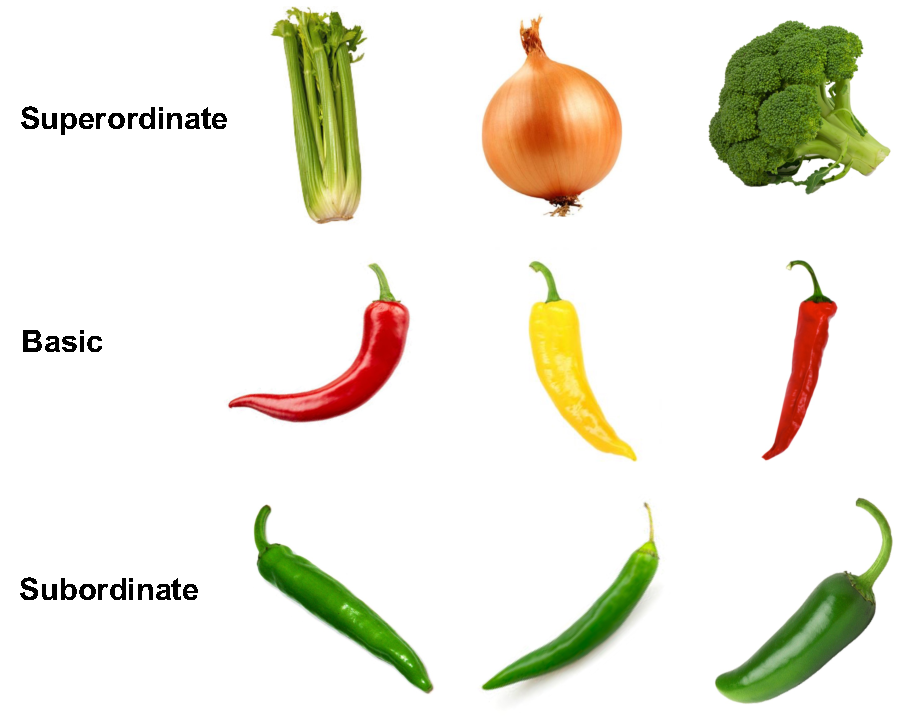
\includegraphics[width=0.5\linewidth]{figs/stim} 

}

\caption{Sample stimuli. Three superordinate (top), basic (middle), and subordinate (bottom) exemplars from the vegetable category.}\label{fig:unnamed-chunk-1}
\end{figure}

\subsection{Procedure}\label{procedure}

Participants were first introduced to a picture of a character
(\enquote{Mr.~Frog}) and instructions describing the task. They were
told that the character speaks a different language and their job was to
help the character find the toys he wants. Participants then advanced to
the main task, which consisted of a series of 12 trials on separate
screens. On each trial, one or three learning exemplars from one of the
three stimulus categories appeared at the top of the screen, along with
the following instructions: \enquote{Here {[}is a wug/are three wugs{]}.
Can you give Mr.~Frog all of the other wugs?.} Below the learning
exemplars, 24 generalization exemplars (8 from each of the 3 categories)
were displayed in a 4\emph{x}6 grid. The order of generalization
pictures was randomized across trials. Participants were instructed to
select the target category members (\enquote{To give a wug, click on it
below. When you have given all the wugs, click the Next button.}). When
an exemplar was selected, a red box appeared around the picture, and
participants were allowed to change their selections by clicking on the
picture a second time. The learning exemplars remained visible at the
top of the screen during the generalization task. Once they had made
their selections, participants advanced to the next trial by clicking
the \enquote{Next} button.

There were four trial types distinguished by the number and semantic
level of the learning exemplars: one subordinate exemplar, three
subordinate exemplars, three basic exemplars, and three superordinate
exemplars. Each participant completed each trial type for each of the
three stimulus categories (vegetables, vehicles, and animals).

Across 12 experiments, we manipulated four aspects of the trial design
that differed between XT and SPSS (summarized in Table 1): Presentation
timing (simultaneous vs.~sequential), trial order (1-3 vs.~3-1), label
(same vs.~different), and blocking (blocked
vs.~pseudo-random).\footnote{All experiments can be viewed directly in the SI.}
We describe each of these factors in more detail below.

\subsubsection{Presentation Timing}\label{presentation-timing}

Presentation timing was the key, theoretically motivated experimental
design difference between experiments by XT (E1 and
E2)\footnote{XT E1 and E2 differed in the age of participants (adults vs.\ children), but we collapse across this difference for the present analyses.}
and SPSS (E2 and E3). In XT, the learning exemplars were presented
statically and simultaneously, while in SPSS, participants saw a
sequence of individual exemplars with each exemplar visible only for 1s
at a time. In the sequential design, three-exemplar learning trials
displayed pictures at three different locations (left, middle, and
right) in a sequence that repeated twice, for a total of 6s.

We reproduced these design aspects in the simultaneous and sequential
versions of our experiments. In the single-exemplar, sequential trials,
the exemplar appeared (1s) and disappeared (1s) for three repetitions.
The generalization pictures did not appear in the sequential condition
until after the training pictures had appeared for 6 seconds, but
remained visible as participants selected generalization exemplars.

\begin{table}

\begin{threeparttable}
\caption{\label{tab:unnamed-chunk-2}Summary of our 12 experiments.}
\centering
\fontsize{12}{14}\selectfont
\begin{tabular}[t]{crrrrrrr}
\toprule
\multicolumn{2}{c}{ } & \multicolumn{4}{c}{Manipulations} & \multicolumn{1}{c}{ } \\
\cmidrule(l{2pt}r{2pt}){3-6}
Exp. & N & Timing & Order & Blocking & Label & Effect Size & Original 
Exp.\\
\midrule
1 & 50 & simult. & 1-3 & pseudo-random & same & 1.32 [1.24, 1.4] & XT E1/E2\\
2 & 50 & simult. & 1-3 & pseudo-random & same & 1.14 [1.06, 1.22] & XT E1/E2\\
3 & 50 & simult. & 1-3 & pseudo-random & diff. & 1.18 [1.1, 1.26] & \\
4 & 50 & simult. & 3-1 & blocked & diff. & 0.02 [-0.06, 0.1] & SPSS ES1/ES2\\
5 & 50 & simult. & 3-1 & blocked & diff. & -0.06 [-0.14, 0.02] & \\
\addlinespace
6 & 50 & simult. & 3-1 & blocked & same & -0.06 [-0.14, 0.02] & \\
7 & 50 & seq. & 1-3 & pseudo-random & same & 1.43 [1.33, 1.53] & \\
8 & 50 & seq. & 1-3 & pseudo-random & diff. & 1.26 [1.18, 1.34] & \\
9 & 50 & seq. & 1-3 & blocked & diff. & 1.31 [1.23, 1.39] & \\
10 & 50 & seq. & 3-1 & blocked & diff. & -0.43 [-0.51, -0.35] & SPSS E2/E3\\
\addlinespace
11 & 50 & seq. & 3-1 & pseudo-random & same & -0.31 [-0.39, -0.23] & \\
12 & 50 & seq. & 3-1 & blocked & same & -0.2 [-0.28, -0.12] & \\
\bottomrule
\end{tabular}
\begin{tablenotes}
\small
\item [1] N = sample size; Timing = presentation timing (sequential or simultaneous); Order = relative ordering of 1 and 3 subordinate trials; Blocking = trials blocked by category or pseudo-random; Label = same or different label in 1 and 3 trials; Effect size = Cohen's d [95\% CI]; Original Exp. = corresponding experiment from prior literature (XT = Xu \& Tenenbaum (2007a); SPSS =   Spencer, et al. (2011);  E = Main  Experiment; ES = Supplemental Experiment).
\end{tablenotes}
\end{threeparttable}
\end{table}

\subsubsection{Trial order}\label{trial-order}

In XT, the three one-subordinate trials occured first followed by all
other trial types (\enquote{1-3}). In contrast, in SPSS (E2 and E3), the
three-subordinate trials occurred first (\enquote{3-1}). SPSS's
replication of XT's simultaneous design (SPSS E1) showed a single block
of either one-subordinate or three-subordinate first (randomized).

\subsubsection{Labels}\label{labels}

\begin{figure}
\centering
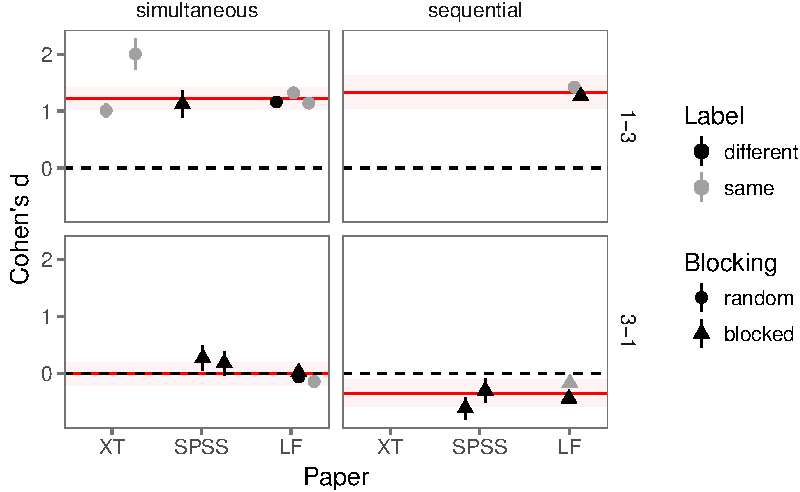
\includegraphics{xtmem_files/figure-latex/unnamed-chunk-3-1.pdf}
\caption{\label{fig:unnamed-chunk-3}Mean proportion generalizations to basic
level exemplars in the one (blue) and three (red) subordinate exemplar
conditions for all 12 of our experiments. Each facet corresponds to a
pairing of presentation timing (simultaneous vs.~sequential) and trial
order (1-3 vs.~3-1). Ranges are bootstrapped 95\% confidence intervals.}
\end{figure}

XT used the same label for each category for the three-subordinate and
one-subordinate trials (e.g., both the single pepper and the
three-pepper trials would be called \enquote{wug}; \enquote{same}). In
contrast, SPSS used a different novel label on each of the 12 trials,
such that the three-subordinate and one-subordinate trials were referred
to with distinct labels (\enquote{different}). We reproduced these two
design choices, and also randomized the mapping of labels to categories
across trials.

\subsubsection{Blocking}\label{blocking}

The studies also differed in whether the trials were blocked by trial
type: In XT, the first three trials were a block of one-subordinate
trials and the remaining 9 were randomized (\enquote{pseudo-random}),
whereas SPSS blocked all four trial types in all experiments
(\enquote{blocked}). We also reproduced these two design variants, while
randomizing trial order within each block for the blocked design.

\begin{figure}
\centering
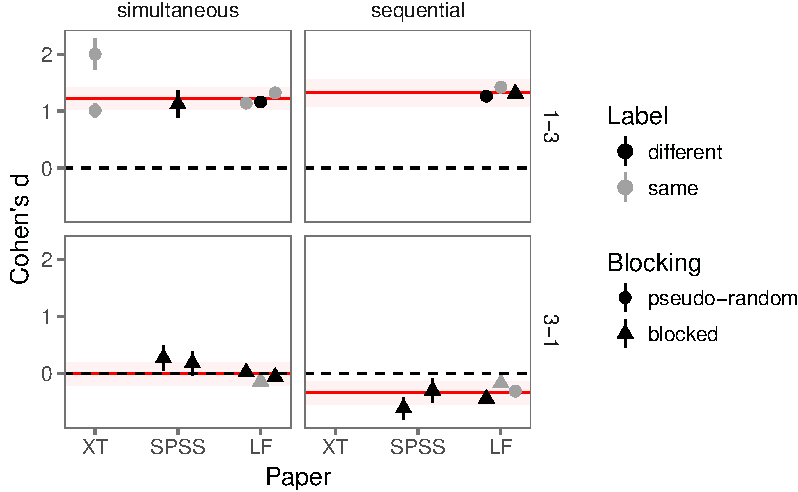
\includegraphics{xtmem_files/figure-latex/unnamed-chunk-4-1.pdf}
\caption{\label{fig:unnamed-chunk-4}Effect sizes for all 19 studies
conducted on the suspicious coincidence effect by XT (Xu \& Tenenbaum,
2007a), SPSS (Spencer, et al, 2011), and the current authors. Top facets
show experiments in which the single exemplar trial occurred first
(1-3); Bottom facets show experiments where the single exemplar trial
occurred second (3-1). Left facets show experiments where exemplars were
presented simultaneously as in XT; Right facets show experiments where
exemplars were presented sequentially as in SPSS. Point color indicates
whether the single exemplar and three subordinate exemplars received the
same (grey) or different (black) label. Point shape indicates whether
trials were blocked by category (circle) or pseudo-random (triangle).
Points are jittered along the x-axis for visibility. The red line
reflects the meta-analytic estimate of the effect size (for the XT
experiments, standard deviations on effect sizes are estimated from the
SPSS replication). All ranges are 95\% confidence intervals.}
\end{figure}

\subsection{Data analysis}\label{data-analysis}

The key prediction of the suspicious coincidence effect is that
participants should generalize to the basic level more often in
one-subordinate trials relative to three-subordinate trials. To measure
this effect, for each trial, we calculated the proportion
generalizations to subordinate exemplars within the same category (out
of 2) and basic exemplars within the same category (out of 2), and
averaged across categories for each participant. We estimated the
difference between the one-subordinate and three-subordinate conditions
by calculating an effect size (Cohen's \emph{d}) for each experiment. We
then estimated the influence of each our design manipulations on the
overall effect size by fitting a random-effect meta-analytic model with
each of our four manipulations as fixed effects. We used the metafor
package (Viechtbauer, 2010) in R to fit our meta-analytic models.

\section{Results}\label{results}

Figure 1 shows the mean proportion generalizations to the basic level in
the one- and three-subordinate trials for all 12
experiments,\footnote{See SI for means across all measures and conditions.}
and Figure 2 shows the corresponding effect sizes (with XT and SPSS
experiments included for reference).

\begin{table}

\caption{\label{tab:unnamed-chunk-5}Meta-analytic model with manipulations as fixed effects.}
\centering
\fontsize{12}{14}\selectfont
\begin{tabular}[t]{lrrr}
\toprule
Fixed effect & beta & z-value & p-value\\
\midrule
Intercept & 1.38 [1.1, 1.66] & 9.55 & <.0001\\
Simultaneous vs. sequential timing & -0.14 [-0.35, 0.07] & -1.32 & 0.19\\
1-3 vs. 3-1 trial order & -1.47 [-1.77, -1.18] & -9.88 & <.0001\\
Different vs. same label & 0.03 [-0.21, 0.27] & 0.26 & 0.8\\
Blocked vs. pseudo-random trial structure & -0.09 [-0.42, 0.23] & -0.56 & 0.58\\
\bottomrule
\end{tabular}
\end{table}

In two exact replications of the XT method, we replicate the suspicious
coincidence effect (Exp. 1: \emph{d} = 1.32 {[}1.24, 1.4{]}; Exp. 2:
\emph{d} = 1.14 {[}1.06, 1.22{]}), with a magnitude comparable to the
original XT experiments (XT E1: \emph{d} = 2 {[}1.73, 2.27{]}; XT E2:
\emph{d} = 1.01 {[}0.89, 1.13{]}). We also replicate the reversal in the
suspicious coincidence effect observed by SPSS in an exact replication
of their method (Exp. 10; \emph{d} = -0.43 {[}-0.51, -0.35{]}), and with
a magnitude comparable to the original experiments (SPSS E2: \emph{d} =
-0.61 {[}-0.81, -0.41{]}; SPSS E3: \emph{d} = -0.3 {[}-0.52, -0.08{]}).

Critically, however, the meta-analytic model across all 12 experiments
reveals that only trial order is a reliable predictor of effect size
(\(\beta\) = -1.47; \emph{Z} = -9.88; \emph{p} \textless{}.0001), while
timing (\(\beta\) = -0.14; \emph{Z} = -1.32; \emph{p} = 0.19), blocking
(\(\beta\) = -0.09; \emph{Z} = -0.56; \emph{p} = 0.58), and label are
not (\(\beta\) = 0.03; \emph{Z} = 0.26; \emph{p} = 0.8; Table 2). These
data thus reveal that the suspicious coincidence is robust to
spatio-temporal aspects of the presentation learning exemplars, in
contrast to the conclusion drawn by SPSS. In the General Discussion, we
consider why trial order might influence the suspicious coincidence
effect.

\section{General Discussion}\label{general-discussion}

The ``suspicious coincidence'' effect (Xu \& Tenenbaum, 2007a) suggests
a powerful mechanism by which learners might overcome the inherent
ambiguity associated with learning subordinate word meanings; Other
evidence (Spencer, Perone, Smith, \& Samuelson, 2011), however, suggests
that the effect may occur only under ecologically invalid learning
conditions---namely, when the training exemplars are presented
simultaneously to the learner. Across 12 studies, we explored the
experimental parameter space of the suspicious coincidence paradigm and
successfully replicated the findings from both sets of authors. Taken
together, our studies lead us to a different conclusion than SPSS: The
suspicious coincidence effect is robust to the presentation timing of
exemplars, but is sensitive to order effects. In particular, we only
observe the suspicious coincidence effect when the single exemplar trial
is presented before the three-exemplar trial.

The critical difference between the 1-3 and 3-1 ordering was the rate of
generalization to the basic level in the one exemplar trial: When the
single exemplar trial occurred second, participants generalized to the
basic level at a much lower rate than in the reverse order. Why might
this ordering matter? We speculate that this difference may be due to
the possibility that learners track exemplar frequency across trials,
due to the pragmatics of the task. In other words, when the single
exemplar trial occurs second, learners may have interpreted this as the
\emph{fourth} exemplar from the same subordinate category in a row,
rather than a single exemplar. This hypothesis predicts that
participants should be less likely to generalize to the basic level on
\enquote{single} exemplar trials compared to three-subordinate trials
under the 3-1 ordering, thus leading to a reversal of the suspicious
coincidence effect. We find some evidence to suggest such a reversal in
an analysis across all experiments with the 3-1 ordering (\emph{t}(581)
= -2.10; \emph{p} = 0.04; \emph{d} = -0.17 {[}-0.19, -0.15{]}).

Our findings highlight the influence of seemingly minor experimental
design parameters on the observed pattern of data. In the present
studies, experiments with the 1-3 versus 3-1 ordering differed by an
effect size of 1.45---a sizable difference that is likely to invite an
unwarranted theoretical explanation. Experimental design parameters are
especially important in the context of replication. When conducting a
replication of an existing finding, small design parameters may
influence the magnitude of the effect (Lewis \& Frank, 2016) and even
its presence (Phillips et al., 2015). This sensitivity requires that
replicators reproduce the original design with as much fidelity as
possible before concluding that an effect fails to replicate. Only then
can the effect be explored, and possible confounds and moderators
identified.

In sum, our studies demonstrate that the suspicious coincidence effect
is robust to a range of experimental parameters, and adds to a growing
body of work suggesting that sampling plays a critical role in learners'
ability to make efficient inferences on the basis of sparse data.

\newpage

\section{References}\label{references}

\setlength{\parindent}{-0.5in} \setlength{\leftskip}{0.5in}

\hypertarget{refs}{}
\hypertarget{ref-bonawitz2011}{}
Bonawitz, E., Shafto, P., Gweon, H., Goodman, N. D., Spelke, E., \&
Schulz, L. (2011). The double-edged sword of pedagogy: Instruction
limits spontaneous exploration and discovery. \emph{Cognition},
\emph{120}(3), 322--330.

\hypertarget{ref-frank2014}{}
Frank, M. C., \& Goodman, N. D. (2014). Inferring word meanings by
assuming that speakers are informative. \emph{Cognitive Psychology},
\emph{75}, 80--96.

\hypertarget{ref-gweon2010}{}
Gweon, H., Tenenbaum, J. B., \& Schulz, L. E. (2010). Infants consider
both the sample and the sampling process in inductive generalization.
\emph{Proceedings of the National Academy of Sciences}, \emph{107}(20),
9066--9071.

\hypertarget{ref-horowitz2016}{}
Horowitz, A. C., \& Frank, M. C. (2016). Children's pragmatic inferences
as a route for learning about the world. \emph{Child Development},
\emph{87}(3), 807--819.

\hypertarget{ref-lawson2014three}{}
Lawson, C. A. (2014). Three-year-olds obey the sample size principle of
induction: The influence of evidence presentation and sample size
disparity on young children's generalizations. \emph{Journal of
Experimental Child Psychology}, \emph{123}, 147--154.

\hypertarget{ref-lawson2017influence}{}
Lawson, C. A. (2017). The influence of task dynamics on inductive
generalizations: How sequential and simultaneous presentation of
evidence impact the strength and scope of property projections.
\emph{Journal of Cognition and Development}.

\hypertarget{ref-lewis2016understanding}{}
Lewis, M. L., \& Frank, M. C. (2016). Understanding the effect of social
context on learning: A replication of Xu and Tenenbaum (2007b).
\emph{Journal of Experimental Psychology: General}, \emph{145}(9),
e72--e80.

\hypertarget{ref-markman1990constraints}{}
Markman, E. M. (1990). Constraints children place on word meanings.
\emph{Cognitive Science}, \emph{14}(1), 57--77.

\hypertarget{ref-phillips2015second}{}
Phillips, J., Ong, D. C., Surtees, A. D., Xin, Y., Williams, S., Saxe,
R., \& Frank, M. C. (2015). A second look at automatic theory of mind:
Reconsidering Kovács, Téglás, and Endress (2010). \emph{Psychological
Science}, \emph{26}(9), 1353--1367.

\hypertarget{ref-shafto2012}{}
Shafto, P., Goodman, N. D., \& Frank, M. C. (2012). Learning from
others: The consequences of psychological reasoning for human learning.
\emph{Perspectives on Psychological Science}, \emph{7}(4), 341--351.

\hypertarget{ref-spencer2011learning}{}
Spencer, J. P., Perone, S., Smith, L. B., \& Samuelson, L. K. (2011).
Learning words in space and time: Probing the mechanisms behind the
suspicious-coincidence effect. \emph{Psychological Science},
\emph{22}(8), 1049--1057.

\hypertarget{ref-tenenbaum2001}{}
Tenenbaum, J., \& Griffiths, T. L. (2001). Generalization, similarity,
and Bayesian inference. \emph{Behavioral and Brain Sciences},
\emph{24}(4), 629--640.

\hypertarget{ref-R-metafor}{}
Viechtbauer, W. (2010). Conducting meta-analyses in R with the metafor
package. \emph{Journal of Statistical Software}, \emph{36}(3), 1--48.
Retrieved from \url{http://www.jstatsoft.org/v36/i03/}

\hypertarget{ref-xu2009}{}
Xu, F., \& Denison, S. (2009). Statistical inference and sensitivity to
sampling in 11-month-old infants. \emph{Cognition}, \emph{112}(1),
97--104.

\hypertarget{ref-xu2007b}{}
Xu, F., \& Tenenbaum, J. B. (2007a). Sensitivity to sampling in Bayesian
word learning. \emph{Developmental Science}, \emph{10}(3), 288--297.

\hypertarget{ref-xu2007word}{}
Xu, F., \& Tenenbaum, J. B. (2007b). Word learning as Bayesian
inference. \emph{Psychological Review}, \emph{114}(2), 245.






\end{document}
